\section{Blur}

\subsection{Introducción}
Blur es un filtro que suaviza la imagen. Esto lo hace asignándole a cada pixel el promedio (media aritmética) con sus pixeles vecinos. Es decir:

% todo: hacer que se vea bien esto...
$m[j][i][k] = (m[j-1][i-1][k] + m[j-1][i][k] + m[j-1][i+1][k] + \\
m[j] [i-1][k] + m[j] [i][k] + m[j] [i+1][k] + \\
m[j+1][i-1][k] + m[j+1][i][k] + m[j+1][i+1][k] ) / 9$

Notar que esto significa que no vamos a procesar los pixeles en los bordes. Esto se debe a que no tienen la cantidad suficiente de pixeles vecinos.

También debemos tener en cuenta el hecho de que a medida que procesemos pixeles, no podemos simplemente pisarlos en memoria. Esto se debe a que un pixel adyacente luego lo puede necesitar para calcular el promedio, por lo que estaríamos mezclando la imagen nueva y la vieja. Hay dos opciones para resolver este problema:
\begin{enumerate}
\item Asignar en memoria un nuevo espacio para guardar los nuevos pixeles. Luego se deben agregar los bordes que no fueron procesados.
\item En primer lugar, guardar las primeras dos filas del la imagen en una nueva posición de memoria. De esa manera podemos pisar los pixeles sobre la imagen original, evitar pedir demasiada memoria y tener que rearmar la imagen al final.
\end{enumerate}
La opción mas elegante y sin lugar a duda correcta es la 2, ya que en términos de construcción y de memoria es mucho mas eficiente.

\subsection{C}
El filtro blur de la cátedra en primer lugar guarda los valores de los pixeles en la primera fila. Arranca en la segunda fila, la copia, y va procesando todos los pixeles de a uno, tomando el promedio de cada componente y reemplazandolo en el mapa de pixeles principal. Esto lo hace por medio de dos loops anidados, uno que recorre las filas, y otro que recorre las columnas. A medida que pasa de fila, intercambia los punteros de la fila recién copiada y la ultima fila copiada. Esto se debe a que cuando pasamos de fila ya no nos interesa saber cuales eran los valores originales dos filas antes. Luego copia la fila actual en el puntero a la fila mas vieja. Se ignora la primera y la ultima fila, y también la primera y la ultima columna. Esto se debe a que no tienen la cantidad suficiente de pixeles vecinos.

Insert pseudo-code here?

\pagebreak

\subsection{ASM1}
Siguiendo la idea del código en C, ASM1 recorre el mapa de pixeles de la misma manera. El código en C procesa cada componente del pixel por separado, mientras que la idea de esta version es procesar todos los componentes de un pixel con SSE. La idea nuevamente es iterar toda la imagen, primero por filas y luego por columnas, reemplazando los pixeles en las posiciones correspondientes.

\begin{table}[h]
\mem
\begin{tabular}{l|c|c|c|c|l}
 & \multicolumn{1}{l|}{}      & \multicolumn{1}{l|}{}       & \multicolumn{1}{l|}{}       & \multicolumn{1}{l|}{}       &  \\ \hline
 & \cellcolor[HTML]{FFCB2F}P1 & \cellcolor[HTML]{FFCB2F}P2  & \cellcolor[HTML]{FFCB2F}P3  & \cellcolor[HTML]{FD6864}P4  &  \\ \hline
 & \cellcolor[HTML]{FFCB2F}P5 & \cellcolor[HTML]{FFFC9E}P6  & \cellcolor[HTML]{FFCB2F}P7  & \cellcolor[HTML]{FD6864}P8  &  \\ \hline
 & \cellcolor[HTML]{FFCB2F}P9 & \cellcolor[HTML]{FFCB2F}P10 & \cellcolor[HTML]{FFCB2F}P11 & \cellcolor[HTML]{FD6864}P12 &  \\ \hline
 & \multicolumn{1}{l|}{}      & \multicolumn{1}{l|}{}       & \multicolumn{1}{l|}{}       & \multicolumn{1}{l|}{}       & 
\end{tabular}
\end{table}
En primer lugar, copiamos la fila correspondiente al contador de filas. Esto da inicio al loop de las filas.

Luego, en el loop de las columnas, buscamos en la copia de la primera fila los 4 pixeles (16 bytes) correspondientes al iterador actual de las columnas. Cada pixel ocupa 32 bits, 1 byte por cada componente ARGB. En la memoria, los archivos $.bmp$ guardan los componentes de los pixeles en el orden A B G R. Como la arquitectura Intel es little-endian, al mover estos pixeles a un registro, no solo se invertira el orden de los pixeles sino que también el de sus componentes.

\mem
\regfloats{$A_1B_1G_1R_1$}{$A_2B_2G_2R_2$}{$A_4B_3G_3R_3$}{$A_4B_4G_4R_4$}

\xmm{1}
\regfloats{$R_4G_4B_4A_4$}{$R_4G_3B_3A_3$}{$R_2G_2B_2A_2$}{$R_1G_1B_1A_1$}

Aquí nosotros hemos levantado 4 pixeles de memoria. Sin embargo notar que para el promedio de los vecinos de un pixel solo necesitamos los 3 primeros. Por lo tanto limpiamos el registro \xmm{1} con un shift a la izquierda y luego uno a la derecha:

\xmm{1}
\regfloats{$0$}{$R_4G_3B_3A_3$}{$R_2G_2B_2A_2$}{$R_1G_1B_1A_1$}

Luego, hacemos las operaciones de empaquetado y desempaquetado para expandir el tamaño de cada componente de pixel de 8 a 16 bits. Esto lo hacemos para que mas adelante cuando tengamos que sumar no tengamos overflow al sumar los componentes de dos pixeles.

\xmm{1}
\regintOcho{$R_2$}{$G_2$}{$B_2$}{$A_2$}{$R_1$}{$G_1$}{$B_1$}{$A_1$}

\xmm{2}
\regintOcho{0}{0}{0}{0}{$R_3$}{$G_3$}{$B_3$}{$A_3$}

Ahora sumamos \xmm{1} y \xmm{2}, poniendo el resultado en \xmm{1}:

\xmm{1}
\regintOcho{$R_2$}{$G_2$}{$B_2$}{$A_2$}{$R_1$+$R_3$}{$G_1$+$G_3$}{$B_1$+$B_3$}{$A_1$+$A_3$}

Repetimos este procedimiento tres veces, uno para cada fila. Finalmente nos queda:

\xmm{1}
\regintOcho{$R_2$}{$G_2$}{$B_2$}{$A_2$}{$R_1$+$R_3$}{$G_1$+$G_3$}{$B_1$+$B_3$}{$A_1$+$A_3$}

\xmm{2}
\regintOcho{$R_6$}{$G_6$}{$B_6$}{$A_6$}{$R_5$+$R_7$}{$G_5$+$G_7$}{$B_5$+$B_7$}{$A_5$+$A_7$}

\xmm{3}
\regintOcho{$R_{10}$}{$G_{10}$}{$B_{10}$}{$A_{10}$}{$R_9$+$R_{11}$}{$G_9$+$G_{11}$}{$B_9$+$B_{11}$}{$A_9$+$A_{11}$}

Ahora sumamos los tres registros en \xmm{1}. Por cuestiones de claridad, lo representamos de a pixeles únicos:

\xmm{1}
\regintOcho{3B}{3G}{3B}{3A}{6R}{6G}{6B}{6A}

Copiamos \xmm{1} en \xmm{2} y lo shifteamos 8 bytes a la derecha:

\xmm{2}
\regintOcho{0}{0}{0}{0}{3B}{3G}{3B}{3A}

Sumando \xmm{1} y \xmm{2} en \xmm{1}:

\xmm{1}
\regintOcho{3B}{3G}{3B}{3A}{9R}{9G}{9B}{9A}

Ahora empaqueto la parte baja del registro para que cada componente de cada pixel pase de 1 a 2 bytes y poder ganar presicion al momento de dividir por 9.

\xmm{1}
\regfloats{9R}{9G}{9B}{9A}

Tomo el promedio de los componentes de cada pixel dividiendo por el registro \regfloats{9.0}{9.0}{9.0}{9.0}.

\xmm{1}
\regfloats{$R_p$}{$G_p$}{$B_p$}{$A_p$}

Finalmente escribo el registro en la posición de memoria correspondiente. Luego incremento el contador de las columnas o de las filas y vuelvo al ciclo correspondiente.

\pagebreak

\subsection{ASM2}

\pagebreak

\subsection{Comentarios}
Al comparar utilizando la imagen de diferencias la imagen generada por el blur de la catedra y la de ASM1, notamos lo siguiente:

\begin{figure}[!htb]
\minipage{0.2\textwidth}
  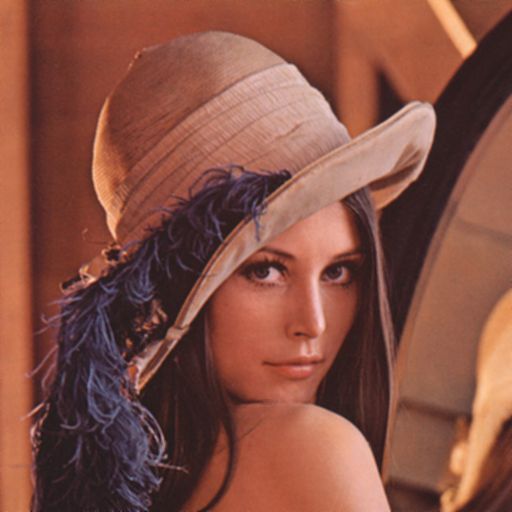
\includegraphics[width=\linewidth]{lenablurc.png}
  \caption{Blur C}
\endminipage\hfill
\minipage{0.2\textwidth}
  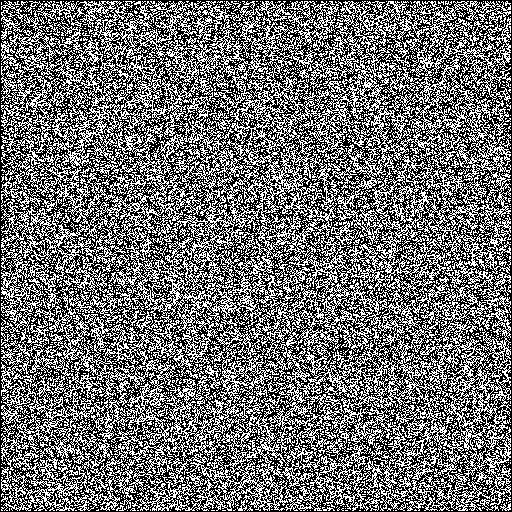
\includegraphics[width=\linewidth]{lenablurdiffR.png}
  \caption{R channel}
\endminipage\hfill
\minipage{0.2\textwidth}
  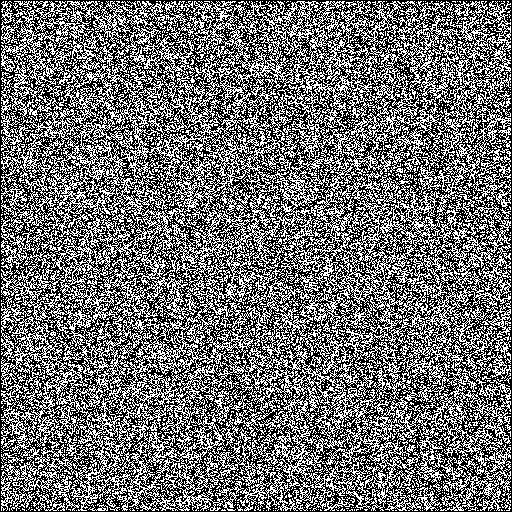
\includegraphics[width=\linewidth]{lenablurdiffG.png}
  \caption{G channel}
\endminipage\hfill
\minipage{0.2\textwidth}
  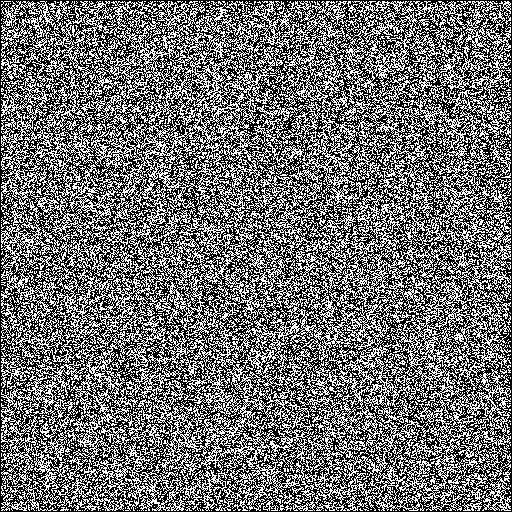
\includegraphics[width=\linewidth]{lenablurdiffB.png}
  \caption{B channel}
\endminipage\hfill
\minipage{0.2\textwidth}%
  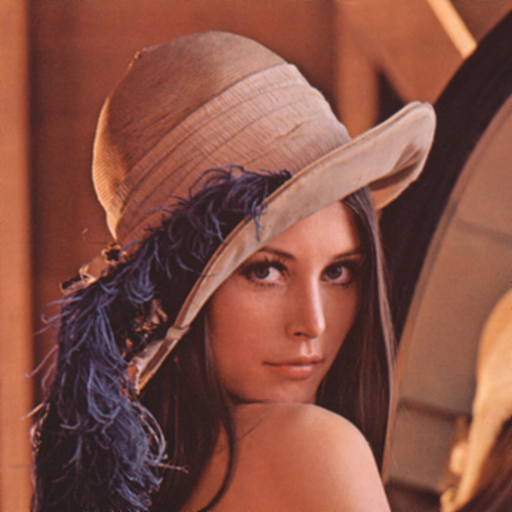
\includegraphics[width=\linewidth]{lenablurasm1.png}
  \caption{Blur ASM}
\endminipage
\end{figure}

Aunque las imágenes parecían exactamente iguales, habían diferencias en algunos pixeles. Estas diferencias se debian al redondeo hacia arriba llevado a cabo por la conversion desde float a entero. Mientras que el codigo en C redondeaba hacia abajo por default, las conversiones en ASM redondeaban hacia arriba por default.

Para resolver esto, existe un flag de SSE llamado $MXCSR$. Para mas información, ver la sección 10.2.3.1 del Volumen 1 de la guía de arquitectura Intel. Cada bit de este flag codifica algún comportamiento de las operaciones SSE. El valor por default de este flag es $0x1F80$. Para que redondee hacia abajo, utilizando la codificación de los bits del flag, había que poner el bit 12 y 13 en 1. Por lo tanto, simplemente setteamos el flag con la instruccion $ldmxcsr$ en $0x7F80$ y empezó a dar perfecto.

